%% LyX 2.0.2 created this file.  For more info, see http://www.lyx.org/.
%% Do not edit unless you really know what you are doing.
\documentclass[english]{report}
\usepackage[latin9]{inputenc}
\usepackage{listings}
\usepackage{textcomp}
\usepackage{amsmath}
\usepackage{amssymb}
\usepackage{graphicx}
\usepackage{esint}
\usepackage{color} %red, green, blue, yellow, cyan, magenta, black, white
\definecolor{mygreen}{RGB}{28,172,0} % color values Red, Green, Blue
\definecolor{mylilas}{RGB}{170,55,241}
% Prova Stile Capitolo
\usepackage[Glenn]{fncychap}

%\makeatletter

%%%%%%%%%%%%%%%%%%%%%%%%%%%%%% LyX specific LaTeX commands.
\DeclareRobustCommand{\greektext}{%
\fontencoding{LGR}\selectfont\def\encodingdefault{LGR}}
\DeclareRobustCommand{\textgreek}[1]{\leavevmode{\greektext #1}}
\DeclareFontEncoding{LGR}{}{}
\DeclareTextSymbol{\~}{LGR}{126}
\newcommand{\lyxmathsym}[1]{\ifmmode\begingroup\def\b@ld{bold}
\text{\ifx\math@version\b@ld\bfseries\fi#1}\endgroup\else#1\fi}

%% Because html converters don't know tabularnewline
\providecommand{\tabularnewline}{\\}
%% A simple dot to overcome graphicx limitations
\newcommand{\lyxdot}{.}


\makeatother
\lstset{language=Matlab,%
    %basicstyle=\color{red},
    breaklines=false,%
    morekeywords={matlab2tikz},
    keywordstyle=\color{blue},%
    morekeywords=[2]{1}, keywordstyle=[2]{\color{black}},
    identifierstyle=\color{black},%
    stringstyle=\color{mylilas},
    commentstyle=\color{mygreen},%
    showstringspaces=false,%without this there will be a symbol in the places where there is a space
    numbers=left,%
    numberstyle={\tiny \color{black}},% size of the numbers
    numbersep=9pt, % this defines how far the numbers are from the text
    emph=[1]{for,end,break},emphstyle=[1]\color{blue}, %some words to emphasise
    %emph=[2]{word1,word2}, emphstyle=[2]{style},    
}
\usepackage{babel}

\begin{document}

\title{Elaborato di Calcolo Numerico}


\author{Finoia Luca  6132811 Calabrese Filippo 5826217 }

\maketitle 

\tableofcontents

% Capitolo 1
\chapter{ERRORI ED ARITMETICA FINITA}
\section{Esercizio 1}
\textit{\textbf{Descrizione:} Verificare che, per h sufficientemente piccolo, $\frac{3}{2}f(x)-2f(x-h)+\frac{1}{2}(x-2h)= hf^{'}(x)+ O(h^{3})$.}\newline

\noindent\emph{Soluzione: }\newline
considerando il Polinomio di Taylor centrato in  $x_{0}$ al secondo ordine:
\begin{equation}
	 f(x_{0} - h) = f(x_{0}) - f^{1}(x_{0})h + \frac{1}{2}f^{2}(x_{0})h^{2}+O(h^{3})
\end{equation}

si effettua una sostituzione con $f(x_{0} - h)$  nella funzione e si ottiene:

\begin{equation}
  \begin{aligned}
      & \frac{2}{3}f(x) - 2\left [ f(x)-f^{1}(x)h+\frac{1}{2}f^{2}(x)h^{2}+O(h^{3}) \right ] + \\
      & +   \frac{1}{2} \left [f(x)-f^{1}(x)2h+\frac{1}{2}f^{2}(x)4h^{2}+O(h^{3})  \right ] = \\
      & = hf^{1}(x)+O(h^{3})
  \end{aligned}
\end{equation}

da cui otteniamo:

\begin{equation}
  \begin{aligned}
      & \frac{3}{2}f(x)-2f(x)+2f^{1}(x)h - \\
      &  - f^{2}(x)h^{2}+\frac{1}{2}f(x) - \\
      &  - f^{1}(x)h+f^{2}(x)h^{2}+O(h^{3}) = \\
      &  = hf^{1}(x)+O(h^{3})
  \end{aligned}
\end{equation}

quindi per h sufficientemente piccoli si ottiene:\newline

\begin{equation}
	 hf^{'}(x)+ O(h^{3}) = hf^{'}(x)+ O(h^{3})
\end{equation}
\newline
\section{Esercizio 2}
\textit{\textbf{Descrizione:} Quanti sono i numeri di macchina normalizzati della doppia precisione IEEE? Argomentare la risposta.}\newline

\emph{Soluzione: }\\~\\
\noindent L'insieme dei numeri di macchina $\mathcal{M}$ \'e un insieme finito di elementi, tramite i quali \'e possibile rappresentare un insieme denso $\mathcal{I}$ e che rappresenta un sottoinsieme dei numeri reali  $\mathcal{I} \subset \mathbb{R}$.

\begin{equation}
	 \mathcal{I} = \left [ -real_{max}, -real_{min}\right ] \cup \left \{  0\right \} \cup \left [real_{min}, real_{max} \right]
\end{equation}

\noindent con $real_{max}$ e $real_{min}$ che indicano rispettivamente il pi\'u grande ed il pi\'u piccolo in valore assoluto tra i numeri macchina diversi da 0.
\\~\\
\noindent Per trovare i numeri di macchina normalizzati che possono essere ottenuti della doppia precisione IEEE possiamo considerare la seguente formula


\begin{equation}
  \begin{aligned}
      b^{s} \cdot b^{m} \cdot (b^{e} - b^{s})\\
  \end{aligned}
\end{equation}

\noindent dove indichiamo con $b$ la base utilizzata, $s$ i bit riservati per il segno, $m$ i bit riservati per la mantissa ed $e$ i bit riservati per l'esponente.
\\~\\
Considerando che lo standard \textit{ANSI/IEEE 754-1985} utilizza una base binaria abbiamo b = 2, inoltre per il formato a doppia precisone abbiamo 1 bit per il segno ($s=1$), 52 bit per la mantissa ($m=52$) e 11 bit per l'esponente ($e=11$),
\\~\\
andando a sostituire i valori appena ricavati nella formula (1.6) otteniamo i numeri di macchina normalizzati che possono essere ottenuti della doppia precisione IEEE, quindi:
\begin{equation}
  \begin{aligned}
      & =  2^{1} \cdot 2^{52} \cdot (2^{11} - 2^{1}) = \\
      & = 2^{1+52} \cdot (2^{11} - 2^{1}) = \\
      & = 2^{1+52+11} - 2^{1+52+1} = \\
      & = 2^{64} - 2^{54} = 18,428,729,675,200,069,632 
  \end{aligned}
\end{equation}
\newpage
\section{Esercizio 3}
\textit{\textbf{Descrizione:} Eseguire il seguente script Matlab e spiegare i risultati ottenuti:
\newline\newline		
format long e\newline
n=75;\newline
u=1e-300; for i=1:n, u=u*2; end, for i=1:n, u=u/2; end, u\newline
u=1e-300; for i=1:n, u=u/2; end, for i=1:n, u=u*2; end, u}\newline

\noindent \textit{\textbf{Svolgimento:}}\newline

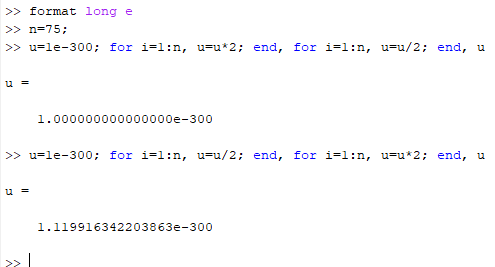
\includegraphics[width=1\linewidth]{img/ex3}
\\~\\
\noindent  in questo script Matlab viene moltiplicato per 2 un valore u=1e-300 per 75 volte, successivamente questo valore u viene diviso per 2 per 75 volte e infine si visualizza il valore in u, poi, viene riportato u al valore di partenza, cio\'e u=1e-300, e viene prima diviso per 2 per 75 volte, poi moltiplicato per 2 per 75 volte  e infine si visualizza il valore in u.
\\~\\
\noindent Se fossimo in matematica esatta, in entrambi i casi, avremmo u che sarebbe uguale al valore di partenza poich\'e \'e stato prima moltiplicato e diviso per la stessa cifra ($2^{75}$) e poi diviso e moltiplicato per la stessa cifra ($2^{75}$). Tuttavia in Matlab i calcoli vengono effettuati in matematica finita e pertanto nel primo caso, in cui la moltiplicazione precede la divisione otteniamo lo stesso risultato che otterremmo in matematica esatta ovvero \text{1.000000000000000e-300}, nel secondo caso invece otteniamo un valore differente ovvero \text{1.119916342203863e-300}.
\\~\\
\noindent La causa per cui nel secondo caso otteniamo un valore diverso da quello iniziale \'e da attribuire ad un errore di round-off, per la precisione un errore di underflow, causato nel primo ciclo in cui viene u viene diviso per 2 per 75 volte, dove, durante una delle iterzioni viene a verificarsi che, $0 < \left | u \right |< r_{min}$ . Essendo che $ r_{min}$ \'e il pi\'u piccolo numero di macchina diverso da zero rappresentabile in valore assoluto, il valore di u viene arrotondato a questo, generando cos\'i un errore di underflow .
\newline
\newline
\section{Esercizio 4}
\textit{\textbf{Descrizione:} Eseguire le seguenti istruzioni Matlab e spiegare i risultati ottenuti:\newline\newline		
format long e\newline
a = 1.111111111111111\newline
b = 1.11111111111111\newline
a + b\newline
a - b}\newline
\newline
\emph{Soluzione: }\\~\\

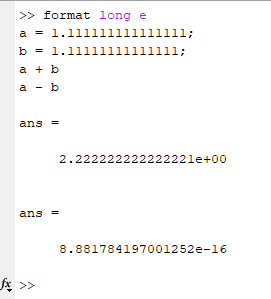
\includegraphics[width=.65\linewidth]{img/ex4}\\~\\
In questo script matlab vengono sommati due numeri $a$ e $b$ e poi viene fatta la differenza tra i due numeri $a$ e $b$.\\~\\
Nel caso della somma tra i due numeri il risultato ottenuto in Matlab corrisponde con il risultato ottenuto in matematica esatta in quanto una somma di numeri concorde \'e sempre ben condizionata poich\'e abbiamo
\begin{equation}
	\left | \varepsilon_{y}  \right | \leq \frac{\left | a \right | + \left | b \right |}{\left | a + b \right |} \varepsilon_{x} \equiv k \cdot \varepsilon_{x}
\end{equation}
in cui k \'e il numero di condizionamento
\begin{equation}
k =  \frac{\left | a \right | + \left | b \right |}{\left | a + b \right |}
\end{equation}
e per una somma di numeri concorde k=1 e quindi \'e sempre ben condizionata.
\\~\\
Nel caso della differenza tra i due numeri $a$ e $b$ invece il risultato ottenuto in Matlab differisce dal risultato ottenuto in matematica esatta perch\'e esso \'e \text{0.000000000000001} . In questo caso si verifica quindi il fenomeno della cancellazione numerica in cui si ha una perdita di cifre significative nel momento in cui viene effettuata una somma tra due numeri prossimi in valore assoluto ma opposti in segno. Infatti in questo caso, in cui $a \approx b$, si ottiene un numero di condizionamento arbitrariamente grande e quindi l'operazione di somma algebrica risulta mal condizionata.

%Capitolo 2 
\chapter{RADICI DI UN EQUAZIONE}
\section{Esercizio 5}

\textit{\textbf{Descrizione:} Scrivere function Matlab distinte che implementino efficientemente i seguenti metodi per la ricerca degli zeri di una funzione:
\begin{itemize}
\item metodo di bisezione 
\item metodo di Newton
\item metodo delle secanti 
\item metodo delle corde
\end{itemize}
Detta $x_{i}$ l'approssimazione al passo i-esimo, utilizzando come criterio di arresto $\left | \Delta x_{i} \right |\leq tol \cdot (1 + \left | x_{i} \right |)$ essendo $tol$ una opportuna tolleranza specificata in ingresso.}\newpage
\emph{Soluzione: }\\~\\
\textbf{il metodo di bisezione:}
\\~\\
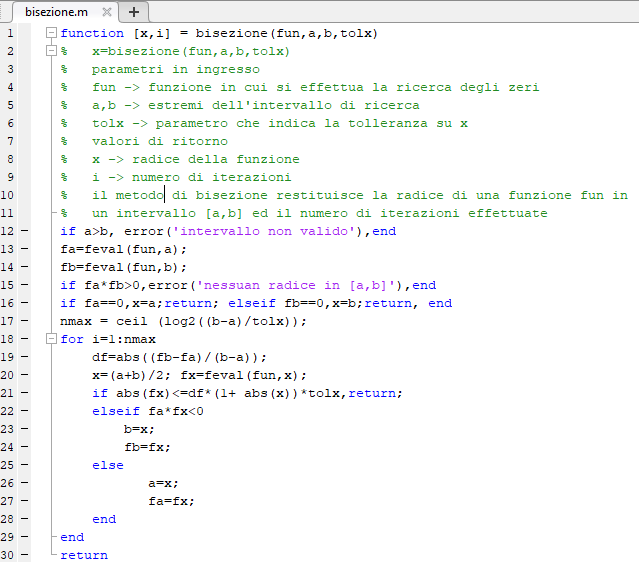
\includegraphics[width=1.3\linewidth]{img/bisezione} \newpage
\textbf{il metodo di Newton:}
\\~\\
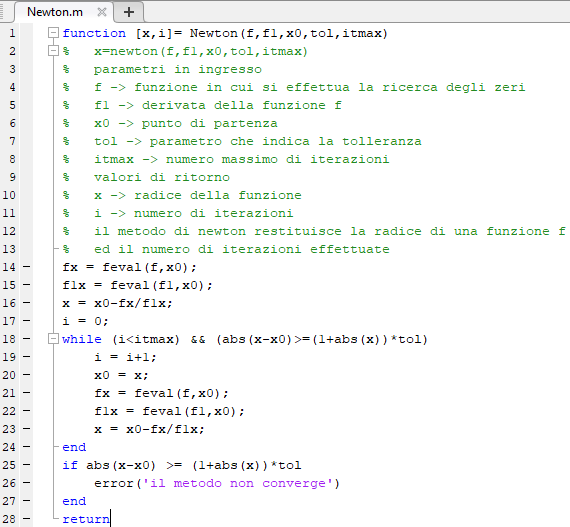
\includegraphics[width=1.3\linewidth]{img/newton}\newpage
\textbf{il metodo delle secanti:}
\\~\\
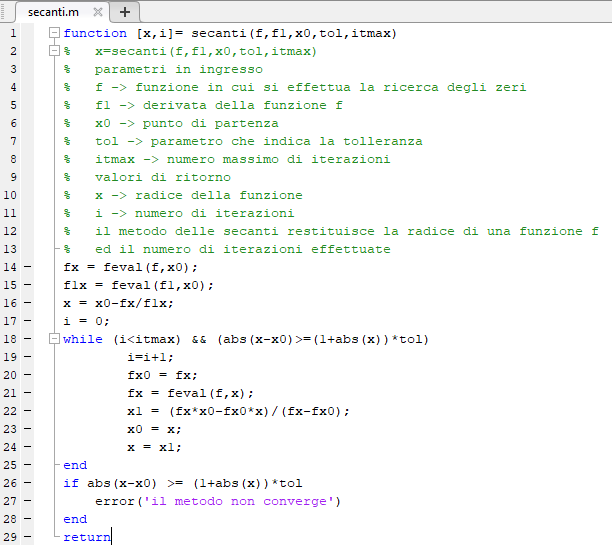
\includegraphics[width=1.3\linewidth]{img/secanti}\newpage
\textbf{il metodo delle corde:}
\\~\\
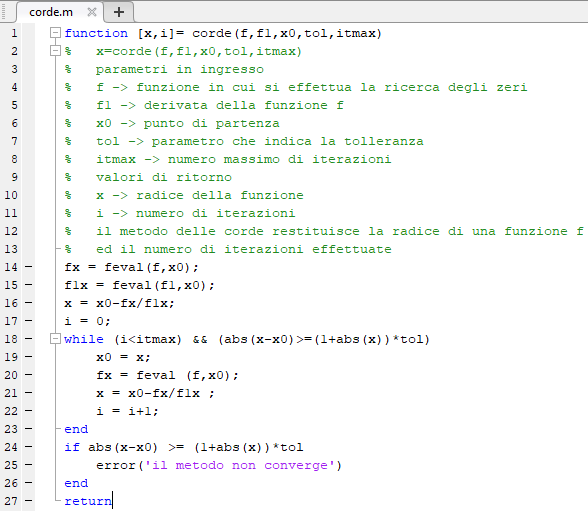
\includegraphics[width=1.3\linewidth]{img/corde}\newpage
\section{Esercizio 6}

\textit{\textbf{Descrizione:} Utilizzare le function del precedente esercizio per determinare una approssimazione della radice della funzione
$f(x) = x - e^{-x}cos(x/100)$,  per $tol = 10^{-i}, \quad i=1, 2,...,12$, partendo da $x_{0} = -1$. Per il metodo di bisezione,
utilizzare $[-1, 1]$, come intervallo di confidenza iniziale. Tabulare i risultati, in modo da confrontare le iterazioni richieste da ciascun metodo. Commentare il relativo costo computazionale.}\\~\\
\emph{Soluzione: }\\~\\

\makebox[\textwidth][c]{
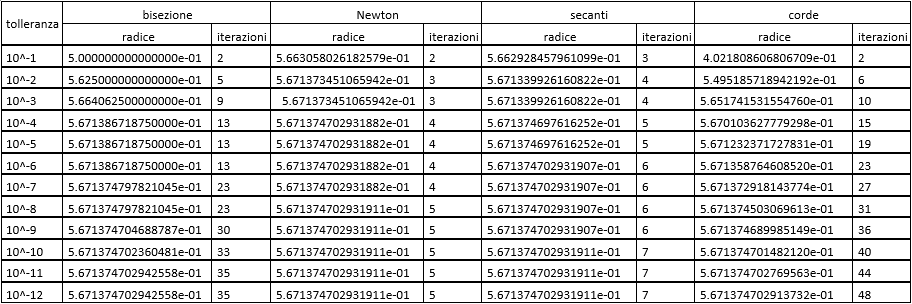
\includegraphics[width=1.3\textwidth]{img/tabella}
}
\\~\\
Nella tabella sono riportate le radici ricavate con ogni metodo e il relativo numero di iterazioni necessarie per ottenere tale risultato per ogni $tol = 10^{-i}, \quad \newline i=1, 2,...,12$.\newline
Il metodo di bisezione ed il metodo delle corde hanno una valutazione di funzione e convergenza lineare mentre il metodo di Newton ha due valutazioni di funzioni, una per la funzione e una per la sua derivata, e convergenza quadratica. Da quanto detto, consegue che col metodo di Newton si ha una maggiore velocit\'a nella ricerca della radice ma si ha anche un costo computazionale maggiore per singola iterazione. Il metodo delle secanti ha una valutazione di funzione, quindi un costo computazionale minore del metodo di Newton,  e una convergenza $\approx$ 1.618, quindi ha una velocit\'a maggiore dei metodi di bisezione e delle secanti.
\section{Esercizio 7}

\textit{\textbf{Descrizione:} Calcolare la molteplicit\'a della radice nulla della funzione $f(x) = x^{2} \cdot sin(x^{2})$. Confrontare, quindi, i metodi di Newton, Newton modificato, e di Aitken, per approssimarla per gli stessi valori di tol del precedente esercizio (ed utilizzando il medesimo criterio di arresto), partendo da $x_{0}=1$. Tabulare e commentare i risultati ottenuti.}\\~\\
\emph{Soluzione:}\\~\\
La molteplicit\'a $m$ della radice nulla della funzione $f(x) = x^{2} \cdot sin(x^{2})$  \'e $m=4$. Per calcolarla, \'e stato utilizzato il seguente script matlab:
\\~\\

\section*{Calcolo della Molteplicit\'a}

\lstinputlisting{resources/molteplicita.m}\newpage

\section*{metodo di  Newton modificato}

\lstinputlisting{resources/NewtonMod.m}\newpage

\section*{metodo di Aitken}

\lstinputlisting{resources/aitken.m}\newpage

\makebox[\textwidth][c]{
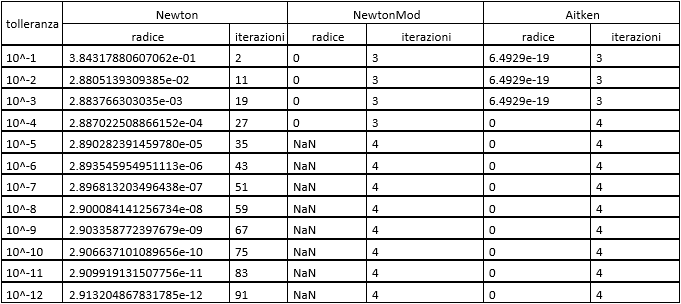
\includegraphics[width=1.3\textwidth]{img/tabella2}
}
\\~\\
dai risultati in tabella si evince che il metodo di Newton richiede un numero elevato di iterazioni nel caso di radici multiple, diventando inefficiente in confronto al metodo di Newton modificato e il metodo di Aitken che richiedono un numero di iterazioni molto minore e risultando cos\'i pi\'u efficienti nel caso di radici multiple ripristinando la convergenza quadratica.%da ricontrollare
% Capitolo 3
\chapter{SISTEMI LINEARI E NON LINEARI}
\section{Esercizio 8}
\textit{\textbf{Descrizione:} Scrivere una function Matlab che, data in ingresso una matrice \textbf{A}, restituisca una matrice, \textbf{LU}, che contenga l'informazione sui suoi fattori \textbf{L} ed \textbf{U}, ed un vettore \textbf{p} contenente la relativa permutazione, della fattorizzazione LU con pivoting parziale di A: \textbf{function [LU,p] = palu(A)}. Curare particolarmente la scrittura e l'efficienza della function.}\newline

\emph{Soluzione:}\\~\\

\section*{fattorizzazione LU con pivoting parziale}

\lstinputlisting{resources/palu.m}\newpage

\section{Esercizio 9}
\textit{\textbf{Descrizione:} Scrivere una function Matlab che, data in ingresso la matrice \textbf{LU} ed il vettore \textbf{p} creati dalla function del precedente esercizio, ed il termine noto del sistema lineare \textbf{Ax = b}, ne calcoli la soluzione: \textbf{function x = lusolve(LU,p,b)}. Curare particolarmente la scrittura e l'efficienza della function.}\newline

\noindent \textit{\textbf{Svolgimento:}}\newline

\section*{Risoluzione matrice fattorizzata LU}

\lstinputlisting{resources/lusolve.m}\newpage

\section{esercizio 10}
\textit{\textbf{Descrizione:} Scaricare la function cremat che crea sistemi lineari $n \times n$ la cui soluzione \'e il vettore $v = (1 \cdots n)^{T}$. Eseguire, quindi, lo script Matlab (vedere esercizio) per testare le function dei precedenti esercizi. Confrontare i risultati ottenuti con quelli attesi, e dare una spiegazione esauriente degli stessi.}\newline
\noindent\emph{Soluzione: }
\\~\\
Una volta scaricata la funzione cremat
\\~\\

\section*{cremat}
\lstinputlisting{resources/cremat.m}

ed eseguito il seguente script
\\~\\
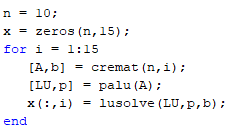
\includegraphics[width=.5\linewidth]{img/ex10.png}
\\~\\
otteniamo i seguenti risultati
\\~\\
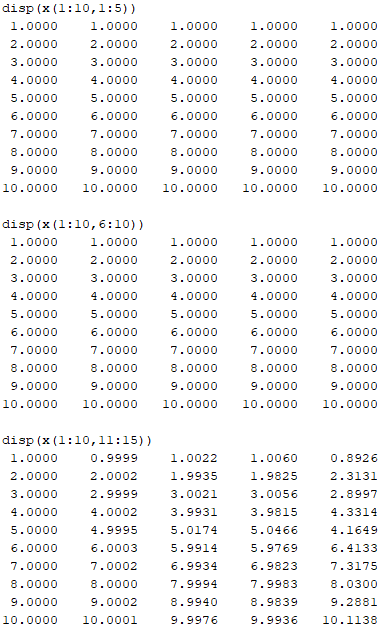
\includegraphics[width=.65\linewidth]{img/tabella10.png}\\~\\
notiamo che i risultati ottenuti coincidono con i risultati attesi per k<12, quindi abbiamo dei risultati perturbati.\newline
Questo vuol dire che per il condizionamento del problema per le matrici

\begin{equation}
	\frac{\left \| \Delta x \right \|}{\left \| x \right \|} \leq k(A)\cdot \left ( \frac{\left \| \Delta b \right \|}{\left \| b \right \|} + \frac{\left \| \Delta A \right \|}{\left \| A \right \|}\right )
\end{equation}
abbiamo un numero di condizionamento di A molto piccolo e quindi una matrice ben condizionata per $1 \leq k<12$ ed un numero di condizionamento di A $>>$ 1 e quindi una matrice mal condizionata per $k \geq 12$
\section{Esercizio 11}
\textit{\textbf{Descrizione:} Scrivere una function Matlab che, data in ingresso una matrice $A \in \mathbb{R}^{m\times n}$, con $m \geq n = rank(A)$, restituisca una matrice, \textbf{QR}, che contenga l'informazione sui fattori \textbf{Q} ed \textbf{R} della fattorizzazione \textbf{QR} di \textbf{A}: \textbf{function QR = myqr(A)}. Curare particolarmente la scrittura e l'efficienza della function.}\newline
\noindent\emph{Soluzione: }\newline
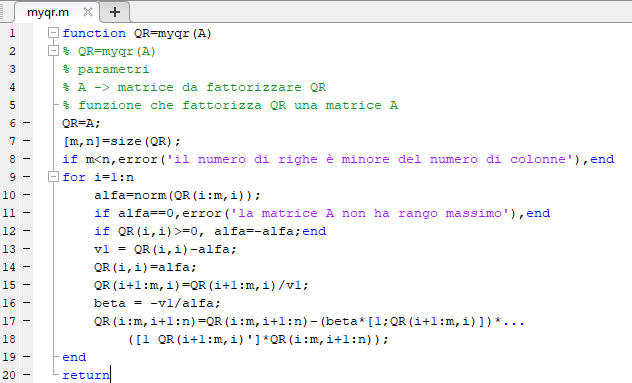
\includegraphics[width=1.3\linewidth]{img/myqr.png}\newpage
\section{Esercizio 12}
\textit{\textbf{Descrizione:} crivere una function Matlab che, data in ingresso la matrice \textbf{QR} creata dalla function del precedente esercizio, ed il termine noto del sistema lineare \textbf{Ax = b}, ne calcoli la soluzione nel senso dei minimi quadrati: function \textbf{x = qrsolve(QR,b)}. Curare particolarmente la scrittura e l'efficienza della function.}\newline
\noindent \textit{\textbf{Svolgimento:}}\newline
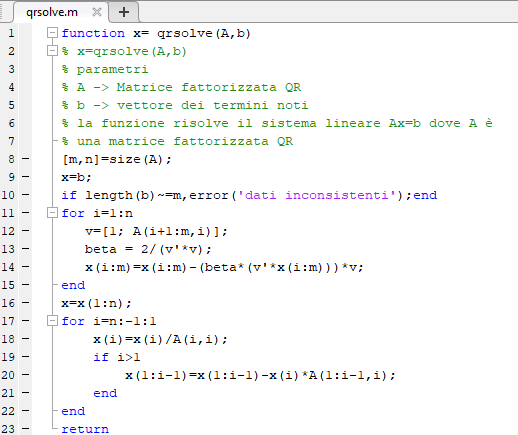
\includegraphics[width=1.3\linewidth]{img/qrsolve.png}\newpage
\section{Esercizio 13}
\textit{\textbf{Descrizione:} Scaricare la function cremat1 che crea sistemi lineari $m \times n$, con $m \geq n$, la cui soluzione (nel senso dei minimi quadrati) \'e il vettore $x = (1 \cdots n)^{T}$. Eseguire, quindi, lo script Matlab (vedere esercizio) per testare le function dei precedenti esercizi.}\newline
\noindent\emph{Soluzione: }\newline
una volta scaricata la function cremat1
\\~\\

\section*{cremat1}

\lstinputlisting{resources/cremat1.m}\newpage

ed aver eseguito lo script\\~\\
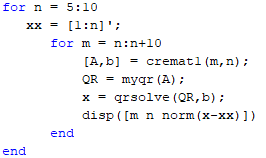
\includegraphics[width=.5\linewidth]{img/ex13.png}\\~\\
otteniamo i seguenti risultati
\\~\\
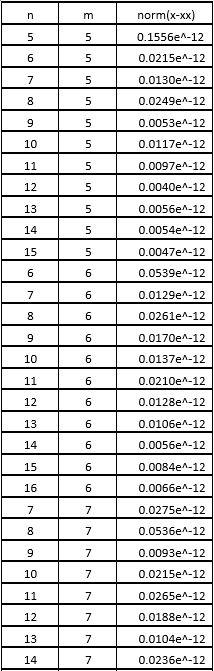
\includegraphics[width=.5\linewidth]{img/tabella13x1.png}\newpage
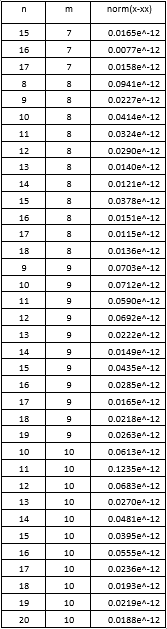
\includegraphics[width=.5\linewidth]{img/tabella13x2.png}
% Capitolo 4
\chapter{APPROSSIMAZIONE DI FUNZIONI}
\section{Esercizio 14}

\textit{\textbf{Descrizione:} Scrivere un programma che implementi efficientemente il calcolo del polinomio interpolante su un insieme di ascisse distinte.}\newline

\noindent\emph{Soluzione: }\newline

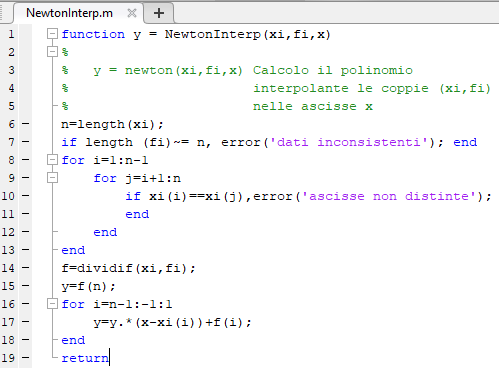
\includegraphics[width=1.3\linewidth]{img/NewtonInter.png}
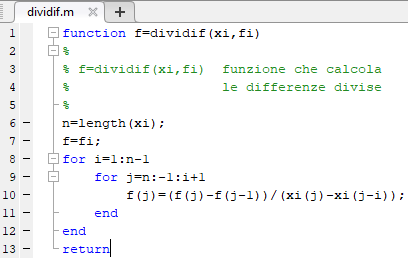
\includegraphics[width=1.3\linewidth]{img/dividif.png}\newpage
\section{Esercizio 15}
\textit{\textbf{Descrizione:} Scrivere un programma che implementi efficientemente il calcolo del polinomio interpolante di Hermite su un insieme di ascisse distinte.}\newline
\noindent\emph{Soluzione: }\newline

\section*{Hermite}

\lstinputlisting{resources/Hermite.m}\newpage
\lstinputlisting{resources/dividifH.m}\newpage
\section{Esercizio 16}
\textit{\textbf{Descrizione:} Scrivere un programma che implementi efficientemente il calcolo di una spline cubica naturale interpolante su una partizione assegnata.}\newline

\noindent\emph{Soluzione: }\newline
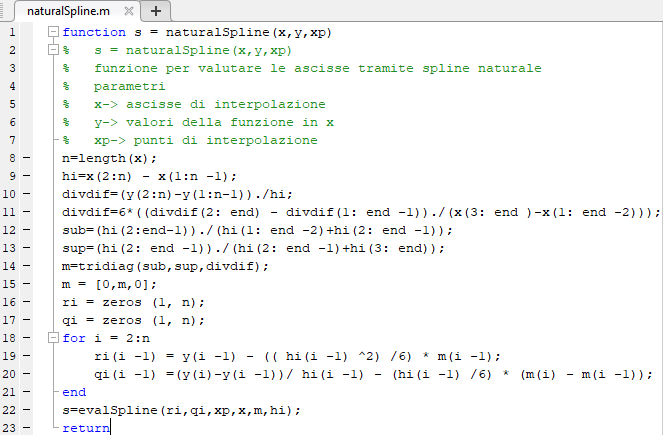
\includegraphics[width=1.3\linewidth]{img/naturalSpline.png}
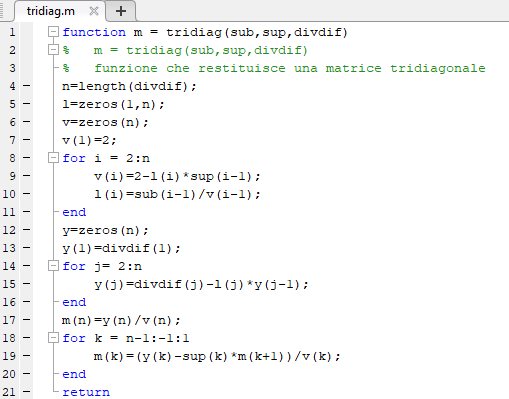
\includegraphics[width=1.3\linewidth]{img/tridiag.png}
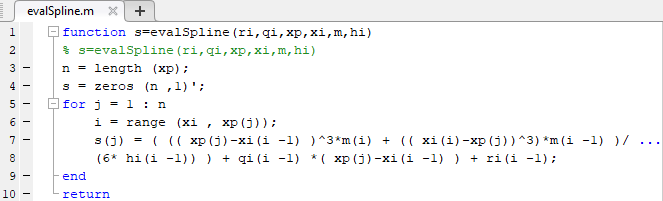
\includegraphics[width=1.3\linewidth]{img/evalSpline.png}
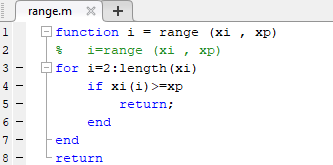
\includegraphics[width=.8\linewidth]{img/range.png}
\section{Esercizio 18}
\textit{\textbf{Descrizione:} Confrontare i codici degli esercizi $14-17$ per approssimare la funzione $f(x) = sin(x)$ sulle ascisse $x_{i} = i \pi/n, i = 0, 1, \cdots , n,$ per $n = 1, 2, \cdots, 10$. Graficare l'errore massimo di approssimazione verso n (in semilogy), calcolato su una griglia uniforme di 10001 punti nell'intervallo $[0, \pi]$.}\newline
\noindent\emph{Soluzione: }\newline
\lstinputlisting{resources/es18.m}
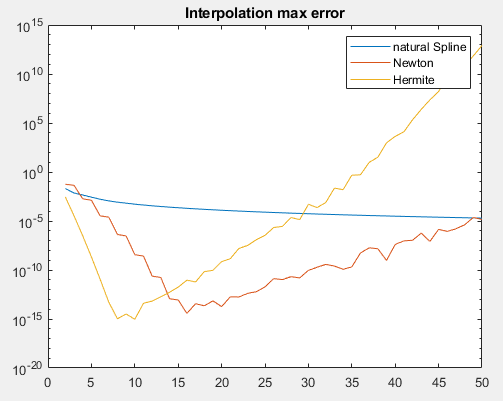
\includegraphics[width=1.3\linewidth]{img/errorInterp.png}%da modificare se viene fatto l'esercizio 17
%Capitolo 5
\chapter{FORMULE DI QUADRATURA}
\section{Esercizio 22}
\textit{\textbf{Descrizione:}  Scrivere due functions che implementino efficientemente le formule adattattive dei trapezi e di Simpson.}\newline
\noindent\emph{Soluzione: }\newline

\section*{formula dei trapezi adattiva}

\lstinputlisting{resources/trapad.m}\newpage

\section*{formula di Simpson adattiva}

\lstinputlisting{resources/simpad.m}\newpage
\section{esercizio 23}
\textit{\textbf{Descrizione:}  Sapendo che}

\begin{equation}
  \begin{aligned}
      & I(x) =\int_{0}^{atan(30)}(1+tan^{2}(x))dx = 30
  \end{aligned}
\end{equation}

\noindent\textit{tabulare il numero dei punti richiesti dalle formule composite dei trapezi e di Simpson per approssimare $I(f)$ con tolleranze $tol=10^{-i}$, con $i = 2,\cdots,8$}
\\~\\
\noindent\emph{Soluzione: }\newline
per prima cosa \'e stato necessario effettuare una modifica al metodo dei trapezi adattivo e al metodo di Simpson adattivo per fare in modo che ritornassero \newline
il numero di punti\\~\\

\lstinputlisting{resources/trapadcount.m}\newpage
\lstinputlisting{resources/simpadcount.m}\newpage
poi si \'e eseguito il seguente script per visualizzare i risultati\newline
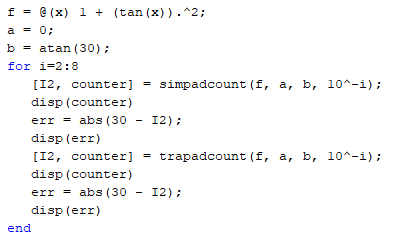
\includegraphics[width=1\linewidth]{img/ex23}\\~\\
ottenendo cos\'i i risultati della seguente tabella\\~\\
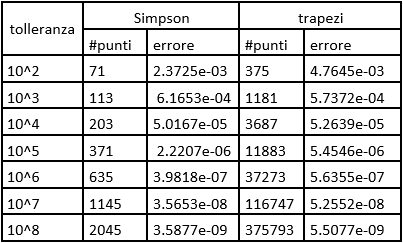
\includegraphics[width=1.3\linewidth]{img/tabella23}

%Capitolo 6
\chapter{CALCOLO DEL GOOGLE PAGERANK}
\section{esercizio 24}
\textit{\textbf{Descrizione:}  Scrivere una function che implementi efficientemente il metodo delle potenze.}\newline
\noindent\emph{Soluzione: }\newline
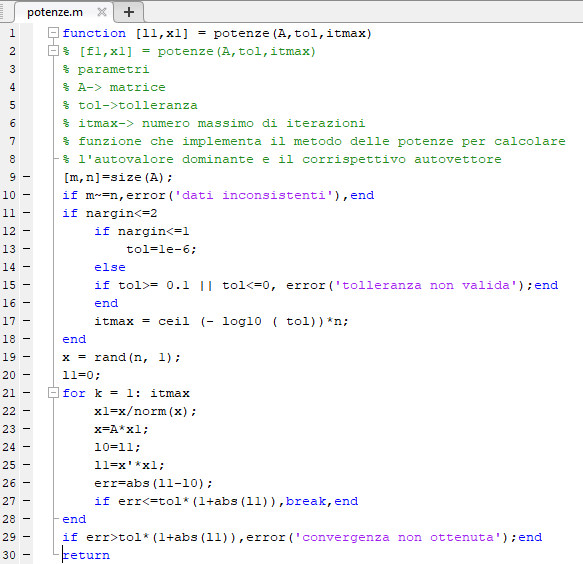
\includegraphics[width=1.3\linewidth]{img/potenze.png}\newpage
\section{Esercizio 25}

\textit{\textbf{Descrizione:}  Sia data la matrice di Toeplitz simmetrica $A_{N}$ in cui le extra-diagonali pi\'u esterne sono le none. Partendo dal vettore $\underline{u}_{0} = (1, \cdots,1)^{T} \in \mathbb{R}^{N}$, applicare il metodo delle potenze con tolleranza $tol=10^{-10}$ per $N=10:10:500$, utilizzando la function dell'esercizio 24. Graficare il valore dell'autovalore dominante, e del numero di iterazioni necessarie per soddisfare il criterio di arresto, rispetto ad N. Utilizzare la funzione spdiags di Matlab per creare la matrice e memorizzarla come matrice sparsa.}

\noindent\emph{Soluzione: }\newline
\section*{metodo delle potenze}
\lstinputlisting{resources/potenzecount.m}\newpage
\lstinputlisting{resources/es25.m}
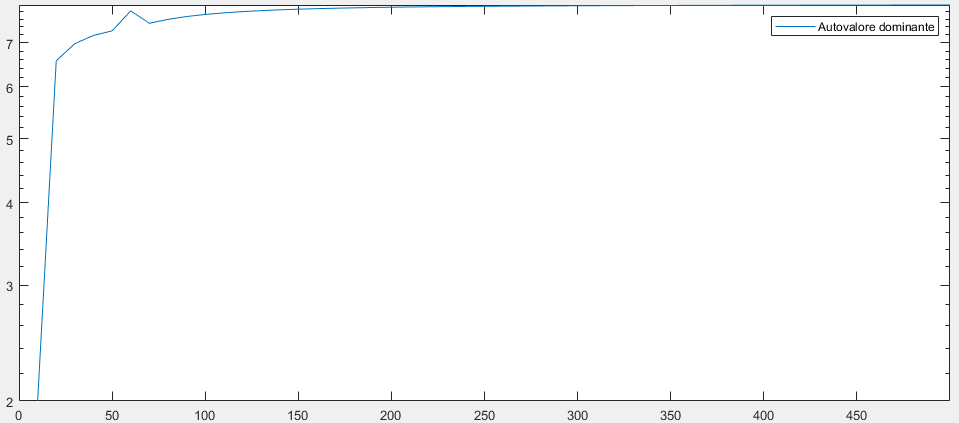
\includegraphics[width=1\linewidth]{img/autovalore.png}
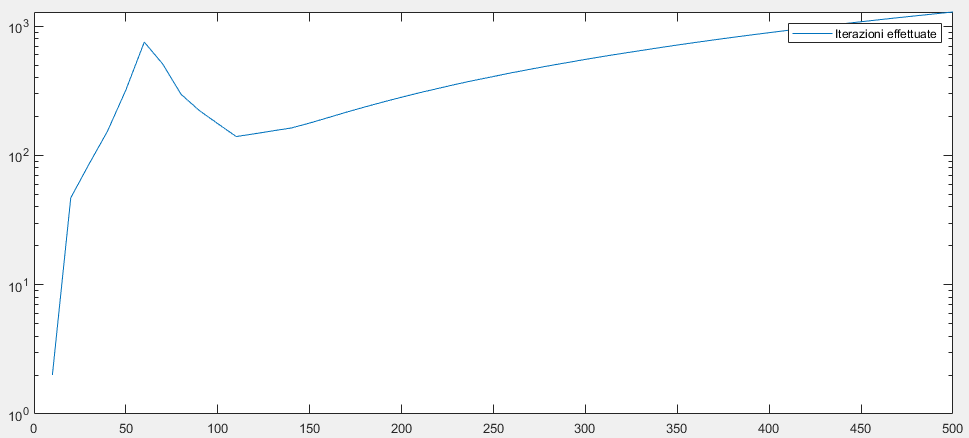
\includegraphics[width=1\linewidth]{img/iterazioniPotenze.png}

\section{Esercizio 26}
\textit{\textbf{Descrizione:}  Scrivere una function che implementi efficientemente un metodo iterativo, per risolvere un sistema lineare, definito da un generico splitting della matrice dei coefficienti.}\newline
\emph{Soluzione: }\\~\\
\textbf{Splitting generico:}
\\~\\
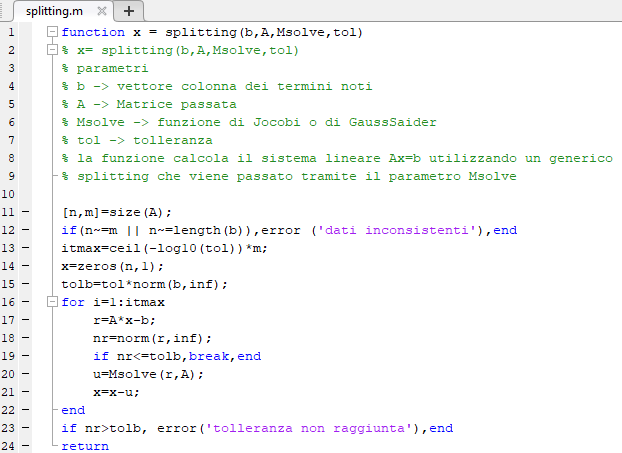
\includegraphics[width=1.3\linewidth]{img/splitting} \newpage
\section{Esercizio 27}
\textit{\textbf{Descrizione:}  Scrivere le function ausiliarie, per la function del precedente esercizio, che implementano i metodi iterativi di Jacobi e Gauss-Seidel.}\newline
\emph{Soluzione: }\\~\\
\section*{il metodo di Jacobi}
\lstinputlisting{resources/Jacobi.m}
\section*{il metodo di GaussSeidel}
\lstinputlisting{resources/GaussSeidel.m}\newpage
\section{Esercizio 28}
\textit{\textbf{Descrizione:}  Con riferimento alla matrice $A_{N}$ definita in $(1)$,  risolvere il sistema lineare $A_{N}x=(1,\cdots,1)^{T}\in \mathbb{R}^{N}$ con i metodi di Jacobi e Gauss-Seidel, per $N = 10:10:500$, partendo dalla approssimazione nulla della soluzione, ed imponendo la norma del residuo sia minore di $10^{-8}$. Utilizzare, a tale fine, la function dell'esercizio 26, scrivendo function ausiliare $ad hoc$ (vedi esercizio 27) che sfruttino convenientemente la struttura di sparsità (nota) della matrice $A_{N}$.  Graficare il numero delle iterazioni richieste dai due metodi iterativi, rispetto ad $N$, per soddisfare il criterio di arresto prefissato.}
\noindent\emph{Soluzione: }\newline
\lstinputlisting{resources/es28/splitting.m}
\lstinputlisting{resources/es28/matvec.m}
\lstinputlisting{resources/es28/jacobi.m}
\lstinputlisting{resources/es28/gaussSeidel.m}
\lstinputlisting{resources/es28/es28.m}
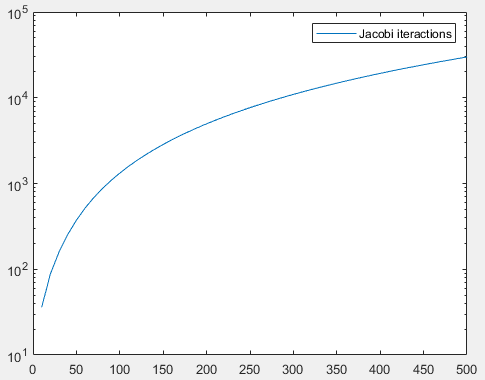
\includegraphics[width=1\linewidth]{img/JacobiIter.png}
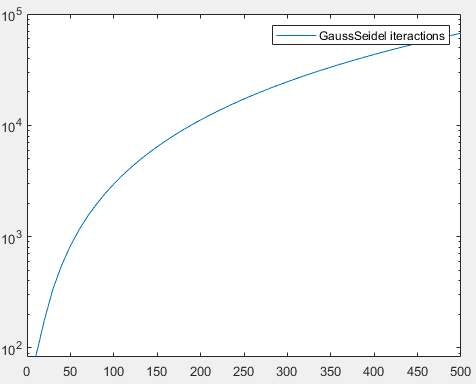
\includegraphics[width=1\linewidth]{img/GSiter.png}

\end{document}
